% !TEX TS-program = pdflatex
% !TeX program = pdflatex
% !TEX encoding = UTF-8
% !TeX spellcheck = en_US

\documentclass{../extra/aakpract/aakpract}

\usepackage{listings}


\settitle{Part-of-Speech tagging}
\setversion{Tutorial}
\setyear{2025-2026}
\setauthor{Dr. Abdelkrime Aries}
\setfooter{Tutorial: PoS tagging}

\begin{document}
	
	\maketitle
	
	\begin{center}
		\begin{minipage}{0.85\textwidth}
			\small\itshape
			This tutorial introduces the main concepts behind sequence labeling in NLP through the example of Part-of-Speech (PoS) tagging. 
			Sequence labeling consists in assigning a label to each token in a sentence while accounting for contextual dependencies between words and labels.
			
			\vspace{6pt}
			The tutorial reviews several modeling approaches, including generative models such as Hidden Markov Models (HMMs), discriminative models like Maximum Entropy Markov Models (MEMMs), and neural architectures based on recurrent neural networks (RNNs) and Transformers. 
			Through analytical questions and decoding exercises, students explore how these models represent contextual information, model label dependencies, and predict the most probable sequence of tags.
			
		\end{minipage}
	\end{center}
	
	
	\section{Quizzes}
	
	\subsection{Quiz}
	
	Select the correct statements:
	
	\begin{longtable}{|p{.95\textwidth}|}
		\hline 
		\Square\ In PoS tagging using an HMM, transitions between states (PoS tags) are modeled as a language model. \\
		\Square\ PoS tagging using an HMM can easily integrate heterogeneous features. \\	
		\Square\ MEMM can use the same features as HMM. \\
		\Square\ MEMM is a discriminative model like HMM. \\
		\hline
	\end{longtable}
	
	
	\subsection{Master 2025/2026 (Modified)}
	
	Among these propositions about sequence labeling, select the correct ones:
	
	\begin{longtable}{|p{.95\textwidth}|}
		\hline 
		\Square\ Sequence labeling can be modeled using a language model over words and another over tags.\\
		\Square\ In NER with BIO tags, the label I-ORG can appear immediately only after B-ORG. \\
		\Square\ In NER, a token tagged as B-PER must represent the first token of a person entity span.\\
		\Square\ In NER, replacing digits with a single symbol ("0") often improves generalization on dates and numbers.\\
		\Square\ In PoS tagging, character-level encoders help handle unseen words by modeling morphology.\\
		\Square\ MEMM operates only on the same features supported by HMM.\\
		\Square\ When training BERT for PoS tagging, the model considers the loss associated with the [PAD] token.\\
		\Square\ In sequence labeling, greedy decoding may create invalid tag sequences.\\
		\Square\ In PoS tagging datasets, the set of possible tags must be known before training.\\
		\Square\ Restricting Viterbi to the K most probable partial paths at each step corresponds to using Beam Search.\\
		\hline
	\end{longtable}
	
	\newpage
	\subsection{Midterm 2024/2025 (Modified)}
	
	Consider this text: 
	
	\textbf{\small\itshape"Eid Mubarak! May this joyous occasion bring you peace, happiness, and prosperity. May your prayers be answered and your heart be filled with gratitude. Wishing you and your loved ones a blessed and joyful Eid! "}
	
	Among these statements about sequence labeling, select the correct ones:
	
	\begin{longtable}{|p{.95\textwidth}|}
		\hline 
		\Square\ The previous text is a good dataset to train Named Entity Recognition (NER) on labels such as organizations, locations, time, etc.\\
		\Square\ When labels correspond to multi-word spans, we can use a mechanism such as IOB to mark the beginning and end, even with Transformer-based models.\\
		\Square\ IOB is the only mechanism to deal with non-atomic parts of a text.\\
		\Square\ MEMM has a limited context like HMM, but it admits more heterogeneous features.\\
		\Square\ For PoS tagging, greedy decoding is the best: it is less complex and more accurate.\\
		\Square\ Beam Search is more efficient than Viterbi when the output space is large, even though it is not exact.\\
		\hline
	\end{longtable}
	
	\subsection{Midterm 2023/2024 (Modified)}
	
	Among these statements about sequence labeling, select the correct ones:
	
	\begin{longtable}{|p{.95\textwidth}|}
		\hline 
		\Square\ "The/\textsubscript{O} UN/\textsubscript{ORG} Security/\textsubscript{ORG} Council/\textsubscript{ORG} on/\textsubscript{O} Monday/\textsubscript{DATE} asked/\textsubscript{O} ..." is the correct annotation for Named Entity Recognition (NER).\\
		\Square\ "The/\textsubscript{O} UN/\textsubscript{B-ORG} Security/\textsubscript{I-ORG} Council/\textsubscript{I-ORG} on/\textsubscript{O} Monday/\textsubscript{B-DATE} asked/\textsubscript{O} ..." is the correct annotation for Named Entity Recognition (NER).\\
		\Square\ If a label does not appear in the training data, we cannot predict it in the test set unless we introduce a \textless UNK\textgreater\ class to detect unknown named entities.\\
		\Square\ If a word does not appear in the training data, we cannot predict whether it belongs to a named entity even if we introduce a \textless UNK\textgreater\ token.\\
		\Square\ For HMM-based PoS tagging, smoothing over transition probabilities is necessary so that unseen tag transitions receive non-zero probability.\\
		\Square\ For RNN-based PoS tagging, transition probabilities are smoothed automatically when there is no overfitting during training.\\
		\Square\ For RNN-based PoS tagging, Viterbi must be used for tag decoding regardless of the architecture.\\
		\hline
	\end{longtable}
	
	Given $T$ words and $N$ possible tags, when using Viterbi to decode the tag sequence, give the most exact complexity:
	
	\begin{center}
		\begin{tabular}{|lllll|}
			\hline
			\Circle\ $ O(2NT) $ & 
			\Circle\ $ O(NT^2) $ & 
			\Circle\ $ O(TN^2) $ & 
			\Circle\ $ O(N+(T-1)N^2) $ & 
			\Circle\ $ O(T+(N-1)T^2) $ \\
			\hline
		\end{tabular}
	\end{center}

	\subsection{Master 2023/2024 (Modified)}
	
	Compare these POS taggers:
	\begin{center}
		\begin{tabular}{|l|c|c|c|c|}
			\cline{2-5}
			\multicolumn{1}{l|}{}
			& HMM & MEMM & RNN & Transformer \\
			\hline
			It learns a language model over POS tags. & \Square & \Square & \Square & \Square \\ 
			\hline
			It does not use the full past context (words/tags). & \Square & \Square & \Square & \Square \\ 
			\hline
			It learns tag dependencies implicitly. & \Square & \Square & \Square & \Square \\
			\hline
		\end{tabular}
	\end{center}
	
	``Viterbi is an exact decoding algorithm for POS tagging.''  
	Is this proposition true or false?
	
	
	\subsection{Midterm 2022/2023 (Modified)}
	
	Compare the following POS tagging methods:
	\begin{center}
		\begin{tabular}{|l|c|c|c|c|}
			\cline{2-5}
			\multicolumn{1}{l|}{}
			& HMM & MEMM & RNN & Transformer \\
			\hline
			Statistical model (non-neural) & \Square & \Square & \Square & \Square \\ \hline
			Can incorporate heterogeneous features & \Square & \Square & \Square & \Square \\ \hline
			Uses an explicit language model & \Square & \Square & \Square & \Square \\
			\hline
		\end{tabular}
	\end{center}
	
	When decoding the POS tags of a given sentence, Beam Search can perform as well as Viterbi in terms of accuracy.
	
	\begin{center}
		\begin{tabular}{|ll|}
			\hline
			\Circle Yes & \Circle No \\
			\hline
		\end{tabular}
	\end{center}
	
	\subsection{Master 2022/2023 (Modified)}
	
	Consider the following French paragraph: 
	
	\textbf{\small\itshape"Débloquer : dégager ou libérer quelque chose. Le déblocage est son action. Exemple : bloquez et débloquez vos cartes SIM. Le sens inverse est le verbe bloquer qui veut dire immobiliser. Un autre sens de ce mot est : grouper en un bloc. La personne qui, lors d’une grève, bloque l’entrée est appelée bloqueur."}
	
	We want to use an MEMM to perform POS tagging on this paragraph. 
	If we want to preserve all useful features of each word for classification, which preprocessing operations should be \textbf{avoided}?
	
	\begin{center}
		\begin{tabular}{|lll|}
			\hline
			\Square\ Tokenization & \Square\ Stemming & \Square\ Stop-words filtering \\
			\Square\ Lowercase normalization & \Square\ Use training treebank & \\
			\hline
		\end{tabular}
	\end{center}
	
	\subsection{Midterm 2021/2022 (Modified)}
	
	Given a sentence with $T$ words and $N$ possible tags, the complexity of the Viterbi algorithm is $O(N^2T)$.
	
	If, at each position $t$, we limit the computation to only the $K < N$ most probable tags from the previous step (beam search), what is the resulting complexity? (The Viterbi matrix will have size $[K, T]$.)
	
	\begin{center}
		\begin{tabular}{|llll|}
			\hline
			\Circle $ O(N^2T) $ & \Circle $ O(KNT) $ & \Circle $ O(K^2T) $ & \Circle $ O(N^2K) $ \\
			\hline
		\end{tabular}
	\end{center}
	
	Can this approach ensure an optimal solution?
	
	\begin{center}
		\begin{tabular}{|ll|}
			\hline
			\Circle Yes & \Circle No \\
			\hline
		\end{tabular}
	\end{center}
	
	
	
	\section{HMM}
	
	\subsection{Master 2025/2026 (Modified)}
	
	Consider a treebank containing the following 4 PoS-annotated sentences: 
	\begin{center}
		\begin{tabular}{|l|l|l|l|}
			\hline
			I/\textsubscript{P} book/\textsubscript{V} a/\textsubscript{D} book/\textsubscript{N} &
			I/\textsubscript{P} fish/\textsubscript{V} a/\textsubscript{D} fish/\textsubscript{N} &
			fish/\textsubscript{N} fish/\textsubscript{V} fish/\textsubscript{N} &
			I/\textsubscript{P} book/\textsubscript{V} a/\textsubscript{D} flight/\textsubscript{N} \\
			\hline
		\end{tabular}
	\end{center}
	
	Using HMM to calculate \textbf{P(P V N \textbar\ I fish fish )}
	
	\begin{center}
		\begin{tabular}{|p{0.3\textwidth}|p{0.2\textwidth}|p{0.2\textwidth}|p{0.2\textwidth}|}
			\hline
			Emission probabilities &&&\\
			\hline
			Initial + Transition probabilities &&&\\
			\hline
		\end{tabular}
	\end{center}
	
	\subsection{Midterm 2024/2025 (Modified)}
	
	Consider a treebank containing the following 4 PoS-annotated sentences:
	\begin{center}
		\begin{tabular}{|ll|}
			\hline
			1) I/\textsubscript{PR} wish/\textsubscript{VB} you/\textsubscript{PR} a/\textsubscript{DT} blessed/\textsubscript{JJ} Eid/\textsubscript{NN} &
			2) I/\textsubscript{PR} hope/\textsubscript{VB} your/\textsubscript{PR} prayers/\textsubscript{NN} are/\textsubscript{VB} answered/\textsubscript{VB} \\
			3) be/\textsubscript{VB} happy/\textsubscript{JJ} and/\textsubscript{CC} peaceful/\textsubscript{JJ} &
			4) have/\textsubscript{VB} a/\textsubscript{DT} joyful/\textsubscript{JJ} Eid/\textsubscript{NN} \\
			\hline
		\end{tabular}
	\end{center}
	
	Using HMM,
	\begin{enumerate}
		\item Calculate the approximate probability \textbf{P(PR VB NN  \textbar\ I enjoyed Eid)}. 
		Show all intermediate calculations (initial, transition, and emission probabilities).
		\item "\textbf{I/\textsubscript{PR} enjoyed/\textsubscript{VB} Eid/\textsubscript{NN}}" is a valid PoS tagging. 
		Propose a method to increase the likelihood of this tag sequence without recomputing all probabilities (be precise about the technique).
		\item Assuming transition and emission probabilities are precomputed and that log probabilities are not used, calculate the number of multiplication operations required to decode the sentence "\textbf{I enjoyed Eid}" using: Greedy decoding, Viterbi decoding, and Brute-force decoding.
	\end{enumerate}
	
	
	\subsection{Master 2024/2025 (Modified)}
	
	Consider a treebank containing the following 4 PoS-annotated sentences:
	\begin{center}
		\begin{tabular}{|l|l|l|l|}
			\hline
			You/\textsubscript{P} light/\textsubscript{V} this/\textsubscript{D} light/\textsubscript{N} &
			they/\textsubscript{P} fish/\textsubscript{V} this/\textsubscript{D} fish/\textsubscript{N} &
			fish/\textsubscript{N} fish/\textsubscript{V} fish/\textsubscript{N} &
			fish/\textsubscript{N} fish/\textsubscript{V} \\
			\hline
		\end{tabular}
	\end{center}
	
	Using an HMM, compute the joint probability: P(You fish this fish \textbar\ P V D N) * P(P V D N)
	
	\begin{center}
		\begin{tabular}{|p{0.3\textwidth}|p{0.1\textwidth}|p{0.1\textwidth}|p{0.1\textwidth}|p{0.1\textwidth}|p{0.1\textwidth}|}
			\hline
			Emission probabilities &&&&&\\
			\hline
			Initial + Transition probabilities &&&&&\\
			\hline
		\end{tabular}
	\end{center}
	
	\subsection{Midterm 2023/2024 (Modified)}
	
	Consider a small treebank containing 4 PoS-annotated sentences:
	\begin{center}
		\begin{tabular}{|l|l|l|l|}
			\hline
			you/\textsubscript{P} light/\textsubscript{V} this/\textsubscript{D} light/\textsubscript{N} &
			they/\textsubscript{P} fish/\textsubscript{V} these/\textsubscript{D} fish/\textsubscript{N} &
			fish/\textsubscript{N} fish/\textsubscript{V} fish/\textsubscript{N} &
			fish/\textsubscript{V} fish/\textsubscript{N} \\
			\hline
		\end{tabular}
	\end{center}
	
	Use an HMM with Laplace smoothing on transition probabilities and consider the probability of the last tag.
	\begin{enumerate}
		\item Calculate the emission probability \textbf{P(these fish light light \textbar\ D N V N)}.
		\item Calculate the exact probability \textbf{P(D N V N \textbar\ these fish light light)} using Bayes' theorem.
	\end{enumerate}
	
	
	\subsection{Master 2023/2024 (Modified)}
	
	We have a treebank (TB) of 3 sentences annotated with nominal phrases (NPs):
	\begin{center}
		\begin{tabular}{|lll|}
			\hline
			[I]\textsubscript{NP} light [the light]\textsubscript{NP} &
			light [the house]\textsubscript{NP} & 
			[You]\textsubscript{NP} lighted [a beautiful torch]\textsubscript{NP} \\
			\hline
		\end{tabular}
	\end{center}
	
	Using an HMM without smoothing, and with Y = belongs to NP, N = not NP (you may encode them differently), calculate:
	
	\begin{center}
		\begin{tabular}{|l|l|l|l|}
			\hline
			\# labels & p(Y $|$ the) & p(Y Y $|$ the torch) & p(Y Y N $|$ the torch light) \\
			\hline
			&&&\\
			\hline
		\end{tabular}
	\end{center}
	
	
	\subsection{Midterm 2022/2023 (Modified)}
	
	Here is a small treebank containing 3 annotated sentences:
	\begin{center}
		\begin{tabular}{|l|l|l|}
			\hline
			I/\textsubscript{P} light/\textsubscript{V} the/\textsubscript{D} torch/\textsubscript{N} &
			You/\textsubscript{P} torch/V the/\textsubscript{D} house/\textsubscript{N} &
			I/\textsubscript{P} house/\textsubscript{V} the/\textsubscript{D} light/\textsubscript{N} \\
			\hline
		\end{tabular}
	\end{center}
	
	\begin{itemize}
		\item Using HMM without smoothing, draw a Viterbi table to PoS-tag the expression "\textbf{You light}" (If a probability is 0, write 0; otherwise provide more detail).
		\item If we want to detect only nominal phrases, describe the procedure and annotate the three sentences accordingly.
	\end{itemize}
	
	
	\subsection{Master 2022/2023 (Modified)}
	
	Here is a small treebank containing 3 annotated sentences:
	\begin{center}
		\begin{tabular}{|l|l|l|}
			\hline
			it/\textsubscript{P} rains/\textsubscript{V} cats/\textsubscript{N} and/\textsubscript{C} dogs/\textsubscript{N} &
			dogs/\textsubscript{N} chase/\textsubscript{V} cats/\textsubscript{N} &
			it/\textsubscript{P} rains/\textsubscript{V} \\
			\hline
		\end{tabular}
	\end{center}
	
	Calculate the following emission, transition, and initial probabilities using an HMM without smoothing:
	\begin{center}
		\begin{tabular}{|l|l|l|l|l|l|}
			\hline
			$ \pi $(N) & P(V $|$ N) & P(N $|$ V) & P(dogs $|$ N) & P(cats $|$ N) & P(chase $|$ V) \\
			\hline
			&&&&&\\
			\hline
			\multicolumn{2}{|l|}{P( N V N $|$ cats chase dogs)} & \multicolumn{4}{|l|}{} \\
			\hline
		\end{tabular}
	\end{center}
	
	\subsection{Midterm 2021/2022 (Modified)}
	
	Here is a treebank of 4 sentences, where each word is annotated with its grammatical category:
	\begin{center}
		\begin{tabular}{|lll|}
			\hline
			I/\textsubscript{PN} fish/\textsubscript{VB} small/\textsubscript{AJ} fish/\textsubscript{NM} &&
			I/\textsubscript{PN} swim/\textsubscript{VB} like/\textsubscript{PR} fish/\textsubscript{NM} \\
			ducks/\textsubscript{NM} swim/\textsubscript{VB} &&
			I/\textsubscript{PN} like/\textsubscript{VB} big/\textsubscript{AJ} fish/\textsubscript{NM} \\
			\hline
		\end{tabular}
	\end{center}
	
	Using an HMM model without smoothing, calculate the probability \textbf{p(NM VB AJ NM $|$ "ducks like small fish")}.
	
	
	\subsection{Master 2021/2022 (Modified)}
	
	The following hidden Markov model illustrates PoS tagging:
	
	\begin{center}
		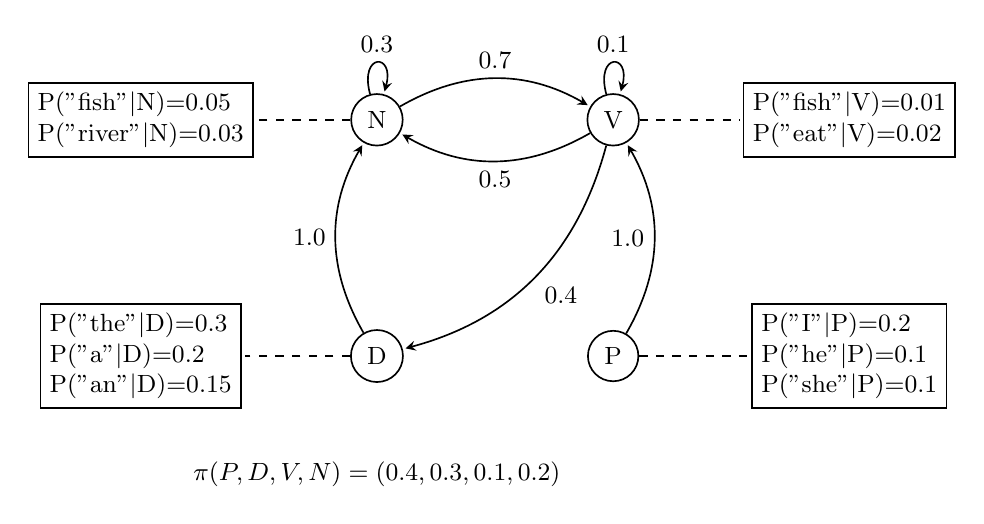
\begin{tikzpicture}[
			> = stealth, % arrow head style
			shorten > = 1pt, % don't touch arrow head to node
			auto,
			node distance = 3cm, % distance between nodes
			semithick, % line style
			font=\small
			]
			
			\tikzstyle{every state}=[
			draw = black,
			thick,
			fill = white,
			minimum size = 4mm
			]
			
			\node[circle,draw] (qN) {N};
			\node[align=left,draw] (qNe) [left of=qN] {P("fish"$|$N)=0.05\\P("river"$|$N)=0.03};
			\node[circle,draw] (qV) [right of=qN] {V};
			\node[align=left,draw] (qVe) [right of=qV] {P("fish"$|$V)=0.01\\P("eat"$|$V)=0.02};
			\node[circle,draw] (qD) [below of=qN] {D};
			\node[align=left,draw] (qDe) [left of=qD] {P("the"$|$D)=0.3\\P("a"$|$D)=0.2\\P("an"$|$D)=0.15};
			\node[circle,draw] (qP) [right of=qD] {P};
			\node[align=left,draw] (qPe) [right of=qP] {P("I"$|$P)=0.2\\P("he"$|$P)=0.1\\P("she"$|$P)=0.1};
			\node[] () [below of=qD, yshift=1.5cm] {$\pi(P, D, V, N) = (0.4, 0.3, 0.1, 0.2)$};
			
			
			\path[->] 	
			(qN) 	edge [loop above] node {0.3} ()
			edge [bend left] node {0.7} (qV)
			(qV) 	edge [loop above] node {0.1} ()
			edge [bend left] node {0.5} (qN)
			edge [bend left] node {0.4} (qD)
			(qD)	edge [bend left] node {1.0} (qN)
			(qP)	edge [bend right] node {1.0} (qV);
			
			\path[dashed] 	
			(qN) 	edge [] node {} (qNe)
			(qV) 	edge [] node {} (qVe)
			(qD) 	edge [] node {} (qDe)
			(qP) 	edge [] node {} (qPe);
			
		\end{tikzpicture}
	\end{center}
	
	\begin{enumerate}
		\item Calculate these two probabilities: \textbf{P(V D N $|$ "fish a fish")} and \textbf{P(N D N $|$ "fish a fish")}
		\item Given C(N) = 200, C(V) = 100 et C(D)=100, calculate these probabilities using Laplace smoothing: \textbf{P(D$|$V)}, \textbf{P(D$|$N)} and \textbf{P(N$|$D)}.
		\item Recalculate the probabilities of the first question using this smoothing.
		\item How many labeled expressions "\textbf{V D N}" exist in our training dataset? 
		Note that the determiner "\textbf{D}" does not occur at the end of a sentence.
	\end{enumerate}
	
	
	\section{MEMM}
	
	\subsection{MEMM Training Exercise}
	
	\begin{center}
		\begin{tabular}{|lll|}
			\hline
			a/\textsubscript{DT} computer/\textsubscript{NN} can/\textsubscript{VB} help/\textsubscript{VB} you/\textsubscript{PN} &&
			he/\textsubscript{PN} can/\textsubscript{VB} swim/\textsubscript{VB}\\
			he/\textsubscript{PN} wants/\textsubscript{VB} to/\textsubscript{TO} help/\textsubscript{VB} you/\textsubscript{PN} &&
			he/\textsubscript{PN} wants/\textsubscript{VB} a/\textsubscript{DT} computer/\textsubscript{NN} \\
			\hline
		\end{tabular}
	\end{center}
	
	\begin{itemize}
		\item Let us use the following features:
		\begin{itemize}
			\item Past, current and future, words encoded using ordinal encoding (alphabetical order)
			\item Past and current PoS encoded using ordinal encoding (alphabetical order)
			\item Binary feature indicating whether the current word has the suffix "s" (1 or 0)
		\end{itemize}
		\item Manually train a MEMM model using these specifications:
		\begin{itemize}
			\item Parameters are initialized to 1; no bias
			\item Instead of \textbf{Softmax}, use \textbf{Average normalization} as activation function
			\item Instead of \textbf{cross entropy} loss, use $J = -\sum_{i=1}^{M} t_i \hat{t}_i$
			\item Learning rate $\alpha=1$ 
			\item 3 iterations
		\end{itemize}
	\end{itemize}
	
	\section{Critical thinking}
	
	\subsection{Master 2025/2026 (Modified)}
	
	For the task below, an architecture is provided. 
	Identify and circle the components that are incorrect or unnecessary, then draw the corrected architecture.

	\begin{center}
		\begin{tabular}{|p{0.4\textwidth}|p{0.4\textwidth}|}
			\hline
			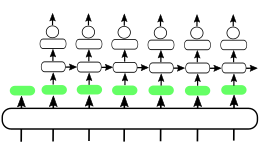
\includegraphics[width=0.4\textwidth]{../img/_tutos/2526_master_arch1a.pdf} &
			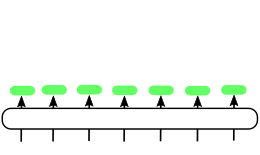
\includegraphics[width=0.4\textwidth]{../img/_tutos/2526_master_arch1b.pdf} \\
			\hline
		\end{tabular}
	\end{center}
	
	Then, identify the corresponding NLP task.
	\begin{center}
		\begin{tabular}{|llllllll|}
			\hline
			\Circle\ Sentiment analysis &
			\Circle\ PoS tagging &
			\Circle\ Paraphrase &
			\Circle\ NER &
			\Circle\ chatbot &
			\Circle\ ATS &
			\Circle\ MT &
			\Circle\ QA \\
			\hline
		\end{tabular}
	\end{center}
	
	
\end{document}
